\chapter{Technische uitvoering}
In wat volgt, worden alle componenten (zowel hardware als software) uitvoerig besproken en wordt een verantwoording gegeven van de ontwerp keuzes.
Dit hoofdstuk wordt opgedeeld in 3 grote onderdelen: lokalisatie, drone aansturing en visualisatie.\\

Op figuur \ref{fig:setup} vindt u de hardware setup, aangevuld met de gebruikte protocollen.\\
\begin{figure}[p]
	\centering
	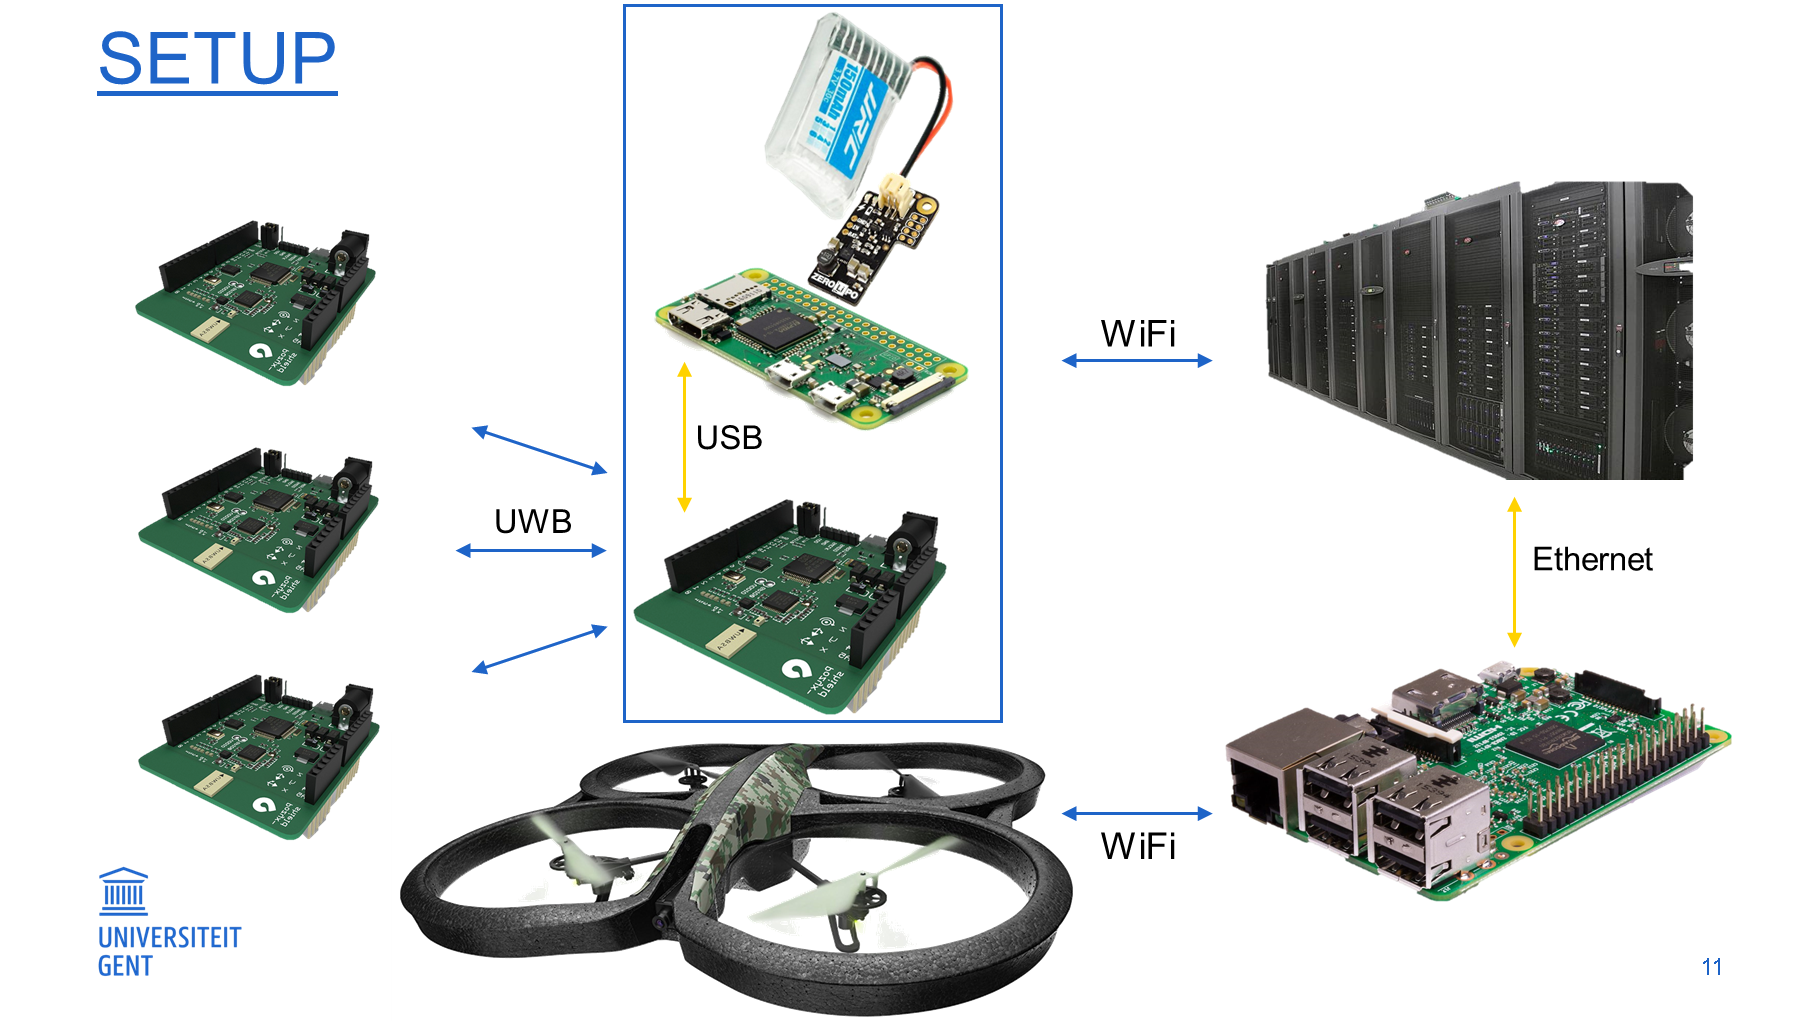
\includegraphics[width=\textwidth]{Setup}
	\caption[Setup]{Hardware setup, aangevuld met protocollen.}
	\label{fig:setup}
\end{figure}

De eerste beslissing omtrent hardware was het uitzoeken van de drone.
Hier werd geopteerd voor de Parrot\footnote{\url{https://parrot.com}} AR.Drone 2.0 Elite Edition met jungle camo.
De belangrijkste argumenten voor deze keuze zijn de kostprijs (\SI{116.71}{\euro{}}), de vluchtduur (\SI{12}{\min}) en het laadvermogen.\\
De meeste types drone die een lading van zo'n \SI{100}{\g} kunnen dragen minstens \SI{250}{\euro{}}.
Dit type is echter al even niet meer in productie, waardoor de prijs enorm gezakt is.
Een goedkopere drone, die niet onder de minidrones geplaatst wordt, kon niet gevonden worden.\\
Ook voor het software gedeelte is deze drone een goede keuze. Parrot stelt een SDK, die toelaat om de drone via wifi aan te sturen en vlucht gegevens op te halen, openbaar ter beschikking.
Er bestaan reeds bibliotheken, waarvan er in dit project ook gebruik gemaakt wordt.\\
De camera op de drone zou kunnen dienen om barcodes in te scannen, maar dat onderdeel werd niet onder de doelstellingen van dit project gedefini\"eerd.\\
Tot slot bezit de drone ook nog een ultrasone sensor om de hoogte t.o.v. de vloer te meten en een camera om stabiel te blijven zweven op dezelfde positie.\\

\section{Lokalisatie}
In theorie is het mogelijk om, als een drone op een gekende locatie (met een gekende ori\"entatie) vertrekt, deze zonder enige input informatie of correcties een reeks vluchtbewegingen door te geven zodat een voorgeprogrammeerde route gevolgd wordt.
In de praktijk wordt dit echter bemoeilijkt door ongekende externe factoren, denk bijvoorbeeld maar aan een ongekend obstakel dat plots het pad van de drone kruist, of een ventilatieschacht die de drone uit positie blaast.
Ook het opstijgen gebeurt niet vlekkeloos, waardoor hij met een foutieve ori\"entatie aan zijn tocht zou beginnen.
Daarom is het nodig dat het toestel z'n specifieke locatie in de ruimte op elk moment gekend is.\\

Als de drone tussen twee rekken met een doorgang van \SI{1}{\m} moet kunnen vliegen, dan moet de nauwkeurigheid van lokalisatie in de grootte orde van \SI{0.10}{\m} liggen.
Veelgebruikte lokalisatie-technologie\"en zoals gps, wifi en bluetooth zijn te onnauwkeurig voor deze toepassing.
Ultra-wideband komt deze noden tegemoet.
Dit is een vrij recente techniek met een nauwkeurigheid in de grootteorde van \SI{0.10}{\m}, wat volstaat om de drone indoor te kunnen lokaliseren.
De locatiebepaling gebeurt via een controller die we op de drone monteren, deze bestaat uit een UWB component, een Raspberry Pi\footnote{\url{https://raspberrypi.org}} Zero W en een batterij.\\

\subsection{UWB component} \label{sec:uwb}
Er werden twee verschillende opties vergelijken (zie tabel \ref{tab:decavspozyx}) als mogelijke UWB component: DecaWave DWM1001 en Pozyx.
De DecaWave is een goedkope, lichte en compacte module.
Echter zou het implementeren van de lokalisatie geen makkelijk programmeer taak zijn, mede doordat de communicatie met de chip niet evident is.
Ook was deze module niet direct beschikbaar. Hierdoor is er gekozen om beroep te doen op de Pozyx-hardware\footnote{\url{https://www.pozyx.io}}, ontwikkeld door een spin-off van de UGent. Deze zijn duurder, zwaarder en groter, maar waren direct beschikbaar en de begeleiders hadden hier al ervaring mee.
Voor de gebruikte drone is het minieme gewichtsverschil van de pozyx tag niet echt een probleem.
Men moet echter wel in het achterhoofd houden dat meer massa de stabiliteit en vliegminuten in negatieve zin be\"invloedt.\\

Op gekende locaties in de ruimte worden Pozyx ankers opgehangen.
De mobiele tag, die onderdeel uit maakt van de controller, kan om de beurt de verschillende ankers aanspreken, en opvragen hoe ver hij van hen verwijderd is.
Deze data wordt dan verwerkt door een Raspberry Pi Zero W.\\

\begin{table}[p]
	\centering
	\begin{tabular}{ | l | c | c | } \hline
		& DecaWave DWM1001 & Pozyx \\
		\hline 
		\hline
		Prijs (\euro{}) & 20 & 135 \\ 
		\hline
		Massa (g) & 4 & 12 \\ 
		\hline
		Afmetingen ($mm \times mm$) & $19.1 \times 26.2$ & $60 \times 53$ \\ 
		\hline
	\end{tabular}
	\caption[Vergelijking DecaWave DWM1001 Module en Pozyx tag]{Vergelijking DecaWave DWM1001 Module en Pozyx tag}
	\label{tab:decavspozyx}
\end{table}

\subsection{Raspberry Pi Zero W} \label{sec:zerow}
Het aansturen van de Pozyx tag gebeurt met een Raspberry Pi Zero W.
De verbinding tussen de Pozyx tag en de Raspberry Pi wordt gelegd via een USB OTG kabel, waarvan beide uiteinden van het type micro-USB zijn.
Deze kleine computer (slechts \SI{9}{\g}) zorgt voor de verwerking van de data die de tag genereert.
Hij is verbonden met het internet en kan zo communiceren met een Mosquitto server die gebruikt wordt voor de verwerking en distributie van de data.
In wat volgt komt deze server nog verder aan bod, hij zorgt voor de connectie van de verschillende onderdelen.
Communicatie met de Mosquitto server werkt via het MQTT-protocol.
Twee belangrijke concepten zijn het \textit{publishen} en het \textit{subscriben} op een bepaalde topic op de server.
Langs de kant van de controller wordt er vooral data verstuurd naar de server (\textit{publish}), terwijl de onderdelen die nog volgen vooral data uitlezen (\textit{subscribe}).\\

De Raspberry Pi stuurt de Eulerhoeken, voor de ori\"entatie van de drone, en de afstanden naar de verschillende ankers naar de server. Door middel van een \textit{particle filter} worden de afstand omgezet naar een precieze locatie.
In dit verslag wordt er niet dieper ingegaan over de berekeningen die hierbij gebeuren.
De visualisatie-software en de software voor het aansturen van de drone luisteren naar deze topics en kunnen deze data verder gebruiken.
Tijdens de start van dit project leverde deze filter de locatie in 2D (intussen ook in 3D), daarom wordt er hier gebruik gemaakt van de ultrasone sensor van de drone voor het bepalen van de hoogte.\\

Naarmate de drone in een groter magazijn rondvliegt, hangen er ook meer ankers.
Een belangrijk aspect naast nauwkeurigheid, is de snelheid waarmee hij zijn locatie kan updaten.
Wanneer de drone zich verplaatste kan het zijn dat hij buiten het bereik is van sommige ankers.
Alle ankers aanspreken zou er dan voor kunnen zorgen dat de update tijd vertraagd.
Een mogelijke manier om dit te verhinderen zou zijn dat de drone enkel de vier ankers aanspreekt die het dichts bij hem in de buurt liggen.

\subsection{LiPo Batterij en Power Supply} \label{sec:lipo}
Een Lithium-ion Polymeer Batterij (LiPo) moet de controller gedurende ongeveer een kwartier van stroom kunnen voorzien, aangezien de drone ook ongeveer \SI{15}{\min} lang in de lucht kan blijven.
De controller heeft gedurende een kwartier ongeveer \SI{350}{\mA} nodig.
Om pieken op te kunnen vangen werd gekozen voor een batterij van \SI{500}{\mA\hour}. Deze kan gedurende een kwartier zo'n \SI{2000}{\mA} leveren aan de controller.\\

Omdat de Rasberry Pi Zero W op \SI{5}{\V} opereert i.p.v. op de \SI{3.7}{\V} van de LiPo batterij, wordt er nog een LiPo SHIM tussen geplaatst.
Deze zal niet enkel het voltage omvormen, maar bezit ook een indicator dat inschakelt wanneer de batterij bijna leeg is.

\section{Drone aansturing} \label{sec:drone_control}
\subsection{Off-board Controller} \label{sec:offboard_controller}
Om de drone effectief aan te sturen maken we gebruik van een Raspberry Pi 3 B.
Deze heeft de mogelijkheid om met 2 netwerken tegelijk te verbinden.
De Ethernet interface wordt gebruikt om verbinding te maken met het internet (en de Mosquitto server), terwijl de wifi interface gebruikt wordt om met het netwerk van de drone te verbinden.\\

Het eerste waarover een beslissing moest genomen worden was het al dan niet gebruiken van een reeds bestaande library, en zo ja de welke?
Bij de keuze van drone werd beschikbaarheid van documentatie reeds in het achterhoofd gehouden waardoor er veel opties beschikbaar waren.
Volgende opties werden onderzocht:
\begin{itemize}
\item python-ardrone
\item YADrone
\item AR Drone Simulink Development-Kit
\item AR Drone Toolkit for LabVIEW
\item Nodecopter
\end{itemize}

Er werd al snel besloten om gebruik te maken van een library, aangezien er hierdoor meer tijd besteed kon worden aan de eigenlijke projectdoelstellingen.
De finale keuze werd gemaakt tussen de python library en Nodecopter.
Doorslaggevend voor de keuze voor Nodecopter was de zeer grote beschikbaarheid van documentatie en extra modules.\\
Aangezien er via Python werd gecommuniceerd zorgde dit er wel voor dat de drone aansturing moest worden opgesplitst in twee delen.
Enerzijds het Node.js deel dat de commando's doorstuurt naar de drone, en anderzijds het python script dat de positie en waypoints ophaalt van de Mosquitto server en omvormt tot instructies voor de drone.

\subsection{Communiceren met de drone via Nodecopter}
Aangezien alle berekeningen reeds worden gedaan in het Python script is de Node.js kant niet veel meer dan een tussenstuk dat alle data ontvangt op een lokale socket en direct doorstuurt naar de drone door middel van Nodecopter commands.
De enige andere noemenswaardige feature is dat het script ook de hoogte zal ontvangen van de drone en dit terugsturen over dezelfde socket.
Dit gebeurd in parallel met de besturingslus zodanig dat deze niet moet wachten op de hoogte.\\

We gebruiken de 'node-ar-drone' library van Nodecopter.
Dit is de standaard library voor het besturen van de drone.
Deze laat toe om de drone high level aan de sturen.
Er kan simpelweg een drone object worden aangemaakt waarop functies als 'forward' of 'left' kunnen opgeroepen worden met als argumenten een fractionele snelheid tussen 0 (stil) en 1 (maximum snelheid).\\

Het gebruik van de 'ardrone-autonomy' library werd ook onderzocht.
Dit is een uitbreiding op de standaard library die toelaat om de drone nog meer high level aan te sturen aan de hand van afstand en draaihoek in plaats van snelheid.
Al snel werd echter duidelijk dat deze library niet accuraat genoeg is  voor binnenvluchten met kleine foutmarges.
\begin{figure}[p]
	\centering
	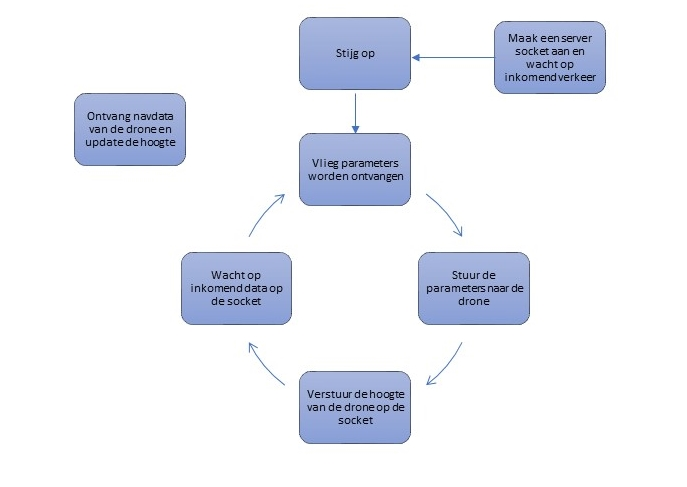
\includegraphics[width=\textwidth]{images/node_server_flowchart}
	\caption[Flowchart van de server]{Flowchart van de server.}
	\label{flowchart_server}
\end{figure}

\subsection{Verwerken van de data in Python}
Het Python script levert het meeste werk.
De locatie verkeregen van de Mosquitto server wordt gebruikt om te berekenen tegen welke snelheid en in welke richting de drone moet vliegen.
Deze informatie wordt dan doorgestuurd over een lokale socket naar het Node.js script op poort 8124.
\begin{figure}[p]
	\centering
	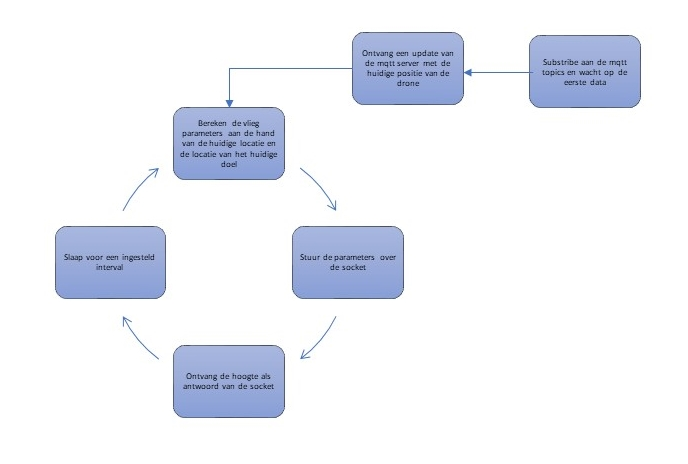
\includegraphics[width=\textwidth]{images/python_client_flowchart}
	\caption[Flowchart van de client]{Flowchart van de client.}
	\label{flowchart_client}
\end{figure}

\subsubsection{Vliegalgoritme 1}
Een eerste poging bestond eruit de informatie omtrent de locatie te gebruiken en om te zetten in twee snelheden, namelijk een voorwaartste snelheid en een hoeksnelheid.
Het idee was simpel: de drone draait zich telkens in de juist richting en gaat dan vooruit.
Hoewel dit idee theoretisch goed klinkt was dit praktisch moeilijker uit te voeren.
Een eerste probleem was dat het vooruit vliegen en draaien parallel gebeurde, wat er dus voor zorgde dat de drone eerder in een boog vloog in plaats van rechtdoor.

\subsubsection{Vliegalgoritme 2}
In een tweede poging werd enkel gebruik gemaakt van de lineare richtingen van de drone, en niet geroteerd.
Het komt er dus op neer dat de drone enkel naar voor, achter, link of rechts gaat, en zijn heading steeds in dezelfde richting wijst.
Dit bleek een accurater algoritme dus hebben we dit verder uitgewerkt.
Een grote beperking in de setup is dat de hoek berekend d.m.v. de Pozyx tags relatief is, en telkens anders is na het opstarten.
Dit heeft als gevolg dat de drone telkens gealligneerd met het assenstelsel moet opstijgen.
Ook hier neemt de snelheid linear af, tot de drone binnen een gegeven afstand van het punt is.
Dan zet hij de parameter 'done' op true, en kan er over gegaan worden naar het volgende waypoint in de lijst.

\section{Visualisatie} \label{sec:visualization}
Unity\footnote{\url{https://unity3d.com/}}.